% Options for packages loaded elsewhere
\PassOptionsToPackage{table}{xcolor}
\PassOptionsToPackage{unicode}{hyperref}
\PassOptionsToPackage{hyphens}{url}
\PassOptionsToPackage{dvipsnames,svgnames,x11names}{xcolor}
\documentclass[
  10pt,
]{article}
\usepackage{xcolor}
\usepackage[margin=1in]{geometry}
\usepackage{amsmath,amssymb}
\setcounter{secnumdepth}{-\maxdimen} % remove section numbering
\usepackage{iftex}
\ifPDFTeX
  \usepackage[T1]{fontenc}
  \usepackage[utf8]{inputenc}
  \usepackage{textcomp} % provide euro and other symbols
\else % if luatex or xetex
  \usepackage{unicode-math} % this also loads fontspec
  \defaultfontfeatures{Scale=MatchLowercase}
  \defaultfontfeatures[\rmfamily]{Ligatures=TeX,Scale=1}
\fi
\usepackage{lmodern}
\ifPDFTeX\else
  % xetex/luatex font selection
\fi
% Use upquote if available, for straight quotes in verbatim environments
\IfFileExists{upquote.sty}{\usepackage{upquote}}{}
\IfFileExists{microtype.sty}{% use microtype if available
  \usepackage[]{microtype}
  \UseMicrotypeSet[protrusion]{basicmath} % disable protrusion for tt fonts
}{}
\makeatletter
\@ifundefined{KOMAClassName}{% if non-KOMA class
  \IfFileExists{parskip.sty}{%
    \usepackage{parskip}
  }{% else
    \setlength{\parindent}{0pt}
    \setlength{\parskip}{6pt plus 2pt minus 1pt}}
}{% if KOMA class
  \KOMAoptions{parskip=half}}
\makeatother
\usepackage{longtable,booktabs,array}
\newcounter{none} % for unnumbered tables
\usepackage{calc} % for calculating minipage widths
% Correct order of tables after \paragraph or \subparagraph
\usepackage{etoolbox}
\makeatletter
\patchcmd\longtable{\par}{\if@noskipsec\mbox{}\fi\par}{}{}
\makeatother
% Allow footnotes in longtable head/foot
\IfFileExists{footnotehyper.sty}{\usepackage{footnotehyper}}{\usepackage{footnote}}
\makesavenoteenv{longtable}
\usepackage{graphicx}
\makeatletter
\newsavebox\pandoc@box
\newcommand*\pandocbounded[1]{% scales image to fit in text height/width
  \sbox\pandoc@box{#1}%
  \Gscale@div\@tempa{\textheight}{\dimexpr\ht\pandoc@box+\dp\pandoc@box\relax}%
  \Gscale@div\@tempb{\linewidth}{\wd\pandoc@box}%
  \ifdim\@tempb\p@<\@tempa\p@\let\@tempa\@tempb\fi% select the smaller of both
  \ifdim\@tempa\p@<\p@\scalebox{\@tempa}{\usebox\pandoc@box}%
  \else\usebox{\pandoc@box}%
  \fi%
}
% Set default figure placement to htbp
\def\fps@figure{htbp}
\makeatother
\setlength{\emergencystretch}{3em} % prevent overfull lines
\providecommand{\tightlist}{%
  \setlength{\itemsep}{0pt}\setlength{\parskip}{0pt}}
\usepackage{newunicodechar}
\newunicodechar{≈}{\ensuremath{\approx}}
\newunicodechar{≥}{\ensuremath{\geq}}
\newunicodechar{∈}{\ensuremath{\in}}
\newunicodechar{→}{\ensuremath{\rightarrow}}
\newunicodechar{×}{\ensuremath{\times}}
\newunicodechar{¹}{\textsuperscript{1}}
\newunicodechar{…}{\ldots}

% --- Table readability ---------------------------------------------------
% Several tables have tall, multi-line cells (the hypothesis scorecard, the
% failure taxonomy, the re-query table). Booktabs alone gives no row
% separators, so adjacent rows blur together. Apply subtle alternating row
% shading + a little extra row height so each row is easy to delimit.
% (The `table` option for xcolor is injected by build.sh before pandoc's own
% \usepackage{xcolor}, which is what makes \rowcolors available here.)
\usepackage{etoolbox}
\definecolor{rowshade}{gray}{0.92}
\AtBeginEnvironment{longtable}{%
  \rowcolors{2}{rowshade}{white}%
  \renewcommand{\arraystretch}{1.18}%
}
\usepackage{bookmark}
\IfFileExists{xurl.sty}{\usepackage{xurl}}{} % add URL line breaks if available
\urlstyle{same}
% fallback for those not using the hyperref driver hyperxmp:
\makeatletter
\@ifundefined{xmpquote}{\newcommand{\xmpquote}[1]{#1}}{}
\makeatother
\hypersetup{
  colorlinks=true,
  linkcolor={blue},
  filecolor={Maroon},
  citecolor={Blue},
  urlcolor={blue},
  pdfcreator={LaTeX via pandoc}}

\author{}
\date{}

\begin{document}

\section{State, Not Tokens: Repository-Scale Agent Reasoning Is Bound by
State
Architecture}\label{state-not-tokens-repository-scale-agent-reasoning-is-bound-by-state-architecture}

\textbf{Cary Palmer}\\
Independent Researcher, Dallas, TX\\
\url{https://github.com/professorpalmer} ·
\url{https://www.linkedin.com/in/cary-palmer-a30557175/}

\textbf{Preprint. All reported numbers are produced by the
machine-checkable oracle and are reproducible from the public code and
data: \url{https://github.com/professorpalmer/durable-state-vs-context}
and
\url{https://huggingface.co/datasets/CaryPalmer/durable-vs-context-trials}.}

\subsection{Abstract}\label{abstract}

The agent community has largely treated repository-scale forgetting as a
\emph{context-window} problem: bigger windows (8k → 128k → 1M) are
expected to yield better whole-repo reasoning. We argue this is a
misdiagnosis. Using a hard, machine-checkable task (strict
JavaScript→TypeScript migration of real OSS repositories under an
unforgeable oracle: strict \texttt{tsc}, immutable test suites,
mandatory \texttt{.js}→\texttt{.ts} replacement, zero
type-escape-hatches), we vary a single axis: \textbf{how state flows
between bounded workers}. Three arms hold model, tools, scaffold, and
oracle constant: a single-context \emph{monolith}, a \emph{durable} arm
that accumulates each completed dependency layer as a committed artifact
on a shared evolving tree, and a \emph{stateless-RAG} arm whose per-file
workers retrieve context but never see each other's results. We find:
(1) a single modern agentic worker already scales much further than the
naive context thesis predicts: it cleanly migrates up to \textbf{240}
interdependent jsdom modules by navigating the filesystem on demand
rather than cramming a working set into the prompt, yet it \textbf{does
crack at the full 364-module tree}, leaving residual strict-type errors
on the hardest module (a \emph{capacity} failure, not a conversion
failure); (2) when work is decomposed for parallelism, \textbf{durable
accumulation strictly dominates stateless retrieval}: RAG's independent
workers emit code that does not even compile (\texttt{TS2451}
redeclaration conflicts appear \emph{only} in RAG), while durable does
not; and (3) durable state confers two structural properties no single
transcript can: \textbf{interruption-resumable consistent checkpoints},
and \textbf{zero-marginal-cost re-query} of any materialized discovery
(a SQLite read, not an LLM call). A failure taxonomy shows three
architectures fail in three distinct ways: RAG by \emph{conflict},
monolith by \emph{capacity}, durable by neither. We also measure the
limit of the parallelism this enables: the dependency critical path
falls to \textbf{4.6\% of total work} at full scale (so headroom
\emph{grows} with repo size), but on the Cursor backend \emph{usable}
concurrency is capped at an effective \textbf{K≈10--12} simultaneous
agent sessions by the serving platform (a replicated n=5--10 sweep with
95\% CIs; success collapses monotonically above the cap). A second
backend (Claude Code) sustains \textbf{100\% to C=32} under the same
orchestrator, confirming the cap is a property of the serving platform,
not of durable state: an orchestration constraint we localize rather
than a limit of the architecture. The contribution is a reframing ---
\emph{state is an asset, not a prompt} --- with controls that isolate
which capability actually matters.

\subsection{1. Introduction}\label{introduction}

The dominant response to repository-scale forgetting in coding agents
has been to enlarge the context window: 8k gave way to 128k gave way to
1M tokens, on the premise that whole-repo reasoning is gated by how much
of the repository fits in the prompt at once (Liu et al., 2023; Packer
et al., 2023). This paper argues that for repository-scale work the
premise is a \emph{misdiagnosis}. A modern agentic worker does not need
to hold the working set in its prompt; it navigates the filesystem on
demand, reading modules as it needs them, and as a result it scales much
further than the naive context-length thesis predicts. Where it
eventually fails, it fails by \emph{capacity} (it cannot maintain global
correctness over the hardest module), not by running out of window. The
binding constraint is \textbf{how state is organized and flows}, not
nominal context length.

The analogy is databases. Scaling was not solved by giving every process
unlimited RAM; it was solved by making the process a \emph{coordinator
over durable state} (indexes, caches, query planners, materialized
views) rather than the \emph{container} of state. A query planner does
not keep the whole table in memory; it reasons over durable structures
and pulls what it needs. We claim repository-scale agents are undergoing
the same transition: the model should be a navigator and reasoner over a
durable, evolving world model of the repository, not a vessel that must
hold the entire working set in a transient prompt and re-derive it every
turn.

The reviewer's sharpest question for any such claim is: \emph{what does
durable state buy that retrieval alone does not?} ``Isn't this just RAG
over a code graph?'' Our answer is mechanistic and measured, not
rhetorical. We hold model, tools, scaffold, and a hardened oracle
constant and vary a single axis (how state flows between bounded
workers) across three arms: a single-context \textbf{monolith}, a
\textbf{durable} arm that accumulates each completed dependency layer as
a committed artifact on a shared evolving tree, and a
\textbf{stateless-RAG} arm whose workers retrieve context but never see
each other's results. RAG \emph{finds} information and throws it away
each turn; durable state \emph{accumulates} discoveries, lets work
decompose across workers without re-derivation, and makes prior findings
consistent and reusable. Those are different capabilities, and the
controlled design isolates them.

\textbf{Contributions.}

\begin{enumerate}
\def\labelenumi{\arabic{enumi}.}
\tightlist
\item
  A controlled study design for repository-scale agents that varies
  \emph{state architecture} with model/tools/oracle held constant, over
  an \emph{unforgeable} oracle (strict \texttt{tsc}, immutable tests,
  mandatory \texttt{.js}→\texttt{.ts} replacement, zero escape hatches)
  and an independent variable of \emph{repository scope}, not prompt
  tokens.
\item
  A refutation of the naive context-length thesis (the single context
  scales cleanly to 240 interdependent modules) and its reframing: the
  single context \emph{does} crack at full-repo scale, but by capacity,
  not window, which sharpens the contribution to ``state architecture,
  not context length.''
\item
  A mechanistic account of \emph{why} durable accumulation beats
  stateless retrieval: a failure taxonomy in which the three
  architectures fail three distinct ways (RAG by \emph{conflict},
  monolith by \emph{capacity}, durable by neither), with \texttt{TS2451}
  redeclaration conflicts appearing \emph{only} in RAG.
\item
  Two structural properties unavailable to any single transcript:
  interruption-resumable consistent checkpoints, and zero-marginal-cost
  re-query of materialized discoveries (a database read, not an LLM
  call).
\item
  An honest localization of the one place durable does \emph{not} win
  (wall-clock at full scale): a \emph{platform} concurrency ceiling
  (K≈10--12 sessions), not state architecture, with the parallel
  headroom shown to \emph{grow} with repo size.
\end{enumerate}

\subsection{2. Related work}\label{related-work}

\textbf{Long-context language models.} A large body of work extends
usable context length and studies its limits. ``Lost-in-the-middle''
effects show that simply enlarging the window does not yield uniform
access to its contents (Liu et al., 2023), and context-management
methods such as MemGPT page information between tiers to fit more useful
signal into a bounded window (Packer et al., 2023). Our results are
complementary but make a different point: for repository-scale coding
the agent need not carry the working set in-window at all. MemGPT still
treats the \emph{window} as the substrate to be fed, whereas we treat
durable committed state as the primary substrate and the window as
incidental, so the relevant axis is state organization, not window size.

\textbf{Retrieval-augmented generation and code-graph retrieval.} RAG
supplies models with relevant context on demand (Lewis et al., 2020),
and repository-level methods such as RepoCoder iterate retrieval and
generation over code (Zhang et al., 2023). We include a stateless-RAG
arm with exactly this capability (per-file workers with code-graph
retrieval) and show that retrieval alone is insufficient when work is
decomposed: without shared, accumulated state, independent workers emit
conflicting declarations that do not compile. The contribution is
precisely to separate \emph{retrieval} (finding context) from
\emph{accumulation} (persisting and reusing discoveries consistently).

\textbf{Agent memory, scratchpads, and external stores.} Prior work
equips agents with memories and reflective stores to persist information
across steps, e.g.~Reflexion's episodic memory of self-critiques (Shinn
et al., 2023) and MemGPT's OS-style memory paging (Packer et al., 2023).
We treat durable state not as an auxiliary memory but as the
\emph{primary computational substrate}: discoveries are committed system
objects on a shared evolving tree, which yields conflict-free
decomposition, resumable checkpoints, and zero-cost re-query: properties
we measure rather than assume.

\textbf{Repository-scale agent benchmarks.} SWE-bench evaluates agents
on real GitHub issues (Jimenez et al., 2023). We differ on three counts:
(i) the independent variable is \emph{state architecture} with
everything else held constant, not end-to-end agent capability; (ii) the
oracle is \emph{unforgeable by construction} (strict typecheck +
immutable tests + mandatory file replacement + zero escape hatches),
eliminating partial credit and hollow passes; and (iii) the scaling
variable is \emph{repository scope} drawn by deterministic BFS over the
dependency graph, so we argue over repo size rather than token budgets.

\subsection{3. Experimental design}\label{experimental-design}

\subsubsection{3.1 Task and oracle}\label{task-and-oracle}

Strict JS→TS migration. Oracle PASS iff:
\texttt{tsc\ -\/-strict\ -\/-noEmit} clean; immutable test suite green;
\textbf{conversion-complete} (no in-scope \texttt{.js} left to shadow a
\texttt{.ts} at runtime); zero escape hatches (\texttt{any},
\texttt{as\ any}, \texttt{@ts-ignore}, \ldots{} budget 0). The oracle
propagates the tsx loader to spawned subprocesses so partial trees load
\texttt{.ts} at runtime. Why this task: success is verifiable and
\emph{adversarially hard to fake}: partial credit and hidden hollow
passes are eliminated by construction.

\subsubsection{3.2 The single varied axis: state
flow}\label{the-single-varied-axis-state-flow}

\begin{itemize}
\tightlist
\item
  \textbf{monolith (C1):} one worker, whole scope, one context.
\item
  \textbf{durable (T):} dependency-layer workers on a shared evolving
  tree; each inherits prior conversions (accumulation ON). Per-layer git
  commit = checkpoint.
\item
  \textbf{stateless-RAG (R):} per-file workers on pristine trees +
  code-graph retrieval, merged at the end (accumulation OFF; reuse only
  by re-derivation).
\end{itemize}

\subsubsection{3.3 Independent variable: repository scope (not
tokens)}\label{independent-variable-repository-scope-not-tokens}

Deterministic BFS over the intra-repo dependency graph from a fixed
anchor, in size strata (jsdom S/M/L/XL/XXL/FULL = 8/24/60/120/240/364,
where FULL is the entire \texttt{lib/} tree). We argue over repo size,
not prompt tokens. Multiple seeds select different scope sets →
generalization.

\subsubsection{3.4 Metrics}\label{metrics}

Oracle pass; wall-clock; worker invocations; peak working set in one
context; escape-hatch count; \textbf{Discovery Reuse Rate (DRR)} =
fraction of dependent in-scope modules whose \texttt{.ts} consumes a
type exported by an already-converted in-scope dependency (a persisted
discovery); failure taxonomy.

\subsubsection{3.5 Serving platform (held constant; one
control)}\label{serving-platform-held-constant-one-control}

All arms run on a single orchestrator (Puppetmaster, dispatching
\textbf{Cursor agent workers}), so the serving platform is held constant
across arms and is \emph{not} the varied axis. Model routing is likewise
fixed. The \textbf{one} exception is §4.8, where we introduce a
\emph{second} backend (\textbf{Claude Code}, Anthropic API) under the
\emph{same} orchestrator purely as a \textbf{control}: it isolates
whether the concurrency ceiling we observe is a property of durable
state (it is not) or of the serving platform (it is). Every other result
in the paper is on the Cursor substrate.

\subsection{4. Results}\label{results}

\subsubsection{\texorpdfstring{4.1 The naive context thesis fails at
moderate scale, but the single context \emph{does} crack at full-repo
scale}{4.1 The naive context thesis fails at moderate scale, but the single context does crack at full-repo scale}}\label{the-naive-context-thesis-fails-at-moderate-scale-but-the-single-context-does-crack-at-full-repo-scale}

{\def\LTcaptype{none} % do not increment counter
\begin{longtable}[]{@{}
  >{\raggedright\arraybackslash}p{(\linewidth - 4\tabcolsep) * \real{0.3333}}
  >{\raggedright\arraybackslash}p{(\linewidth - 4\tabcolsep) * \real{0.3333}}
  >{\raggedright\arraybackslash}p{(\linewidth - 4\tabcolsep) * \real{0.3333}}@{}}
\toprule\noalign{}
\begin{minipage}[b]{\linewidth}\raggedright
scope (jsdom modules)
\end{minipage} & \begin{minipage}[b]{\linewidth}\raggedright
monolith
\end{minipage} & \begin{minipage}[b]{\linewidth}\raggedright
note
\end{minipage} \\
\midrule\noalign{}
\endhead
\bottomrule\noalign{}
\endlastfoot
7 (express) & PASS & \\
8 & PASS & \\
24 & PASS & \\
60 & PASS & 0 hatches, 41 min \\
120 & PASS & 0 hatches, 46 min \\
240 & PASS & 0 hatches, 26 min \\
\textbf{364 (full \texttt{lib/})} & \textbf{FAIL} & converts all, tests
green, 0 hatches, but \textbf{16 strict-type errors} \\
\end{longtable}
}

\begin{figure}
\centering
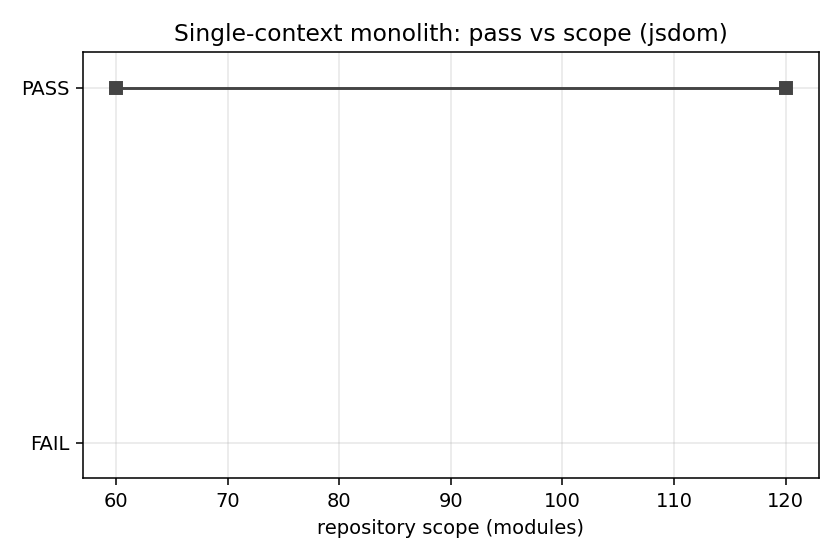
\includegraphics[width=0.72\linewidth,height=\textheight,keepaspectratio,alt={The single-context monolith passes the oracle at every scope up to 240 interdependent modules and fails only at the full 364-module tree, and it fails by capacity (residual strict-type errors on the hardest module), not by window overflow.}]{../figures/monolith_scaling.png}
\caption{The single-context monolith passes the oracle at every scope up
to 240 interdependent modules and fails only at the full 364-module
tree, and it fails by \emph{capacity} (residual strict-type errors on
the hardest module), not by window overflow.}
\end{figure}

A single context did \textbf{not} break where the context-length thesis
predicts (Fig. 1): the agent is \emph{already} a reasoner over external
state (the filesystem), pulling in modules on demand rather than
cramming a working set into the prompt. It cleanly migrated up to
\textbf{240} interdependent modules. \textbf{This is itself a finding}
and it reframes the contribution away from ``state beats context for a
single agent.''

But at the \textbf{full 364-module \texttt{lib/} tree the one-shot
architecture degrades}: it still converts everything and gets the test
suite green with zero escape hatches, yet leaves \textbf{16 residual
strict-type errors} (\texttt{TS2322} assignability ×8, \texttt{TS2571}
``object is of type `unknown'\,'' ×7, \texttt{TS2339} ×1), concentrated
in the single hardest module (\texttt{XMLHttpRequest-impl}). Notably it
failed \emph{safely} (it reached for \texttt{unknown}, not \texttt{any})
but ran out of capacity to globally narrow types at full scale. This is
a \textbf{capacity} failure (correctness under a single global view),
categorically different from RAG's failure mode below.

\textbf{Durable at the same 364 scale (capstone).} Durable decomposition
converted all 364 modules (364 workers, \textasciitilde3.2 h) and its
\emph{raw} tree carries \textbf{only 5 type errors vs the monolith's
16}. We are careful not to overclaim: durable does \textbf{not}
eliminate conflicts outright. Its residue is bounded \emph{intra-layer}:
sibling modules converted in the \textbf{same} dependency layer are
blind to each other (each sees only \emph{prior} committed layers), so
two CSS-rule siblings redeclared a shared type
(\texttt{TS2451}/\texttt{TS2300}). This is the \emph{same conflict
class} RAG suffers, but \textbf{bounded to a single layer} instead of
global. Because the tree is decomposed and consistent, \textbf{targeted
iterative repair} (re-run only the conflicting modules, which can now
see each other on the shared tree) drove the tree to a clean
\texttt{typecheck\_strict} in \textbf{3 iterations / 4 repair-worker
calls / 258 s (\textasciitilde4.3 min)}, verified
\texttt{tsc\ -\/-strict\ -\/-noEmit} 0-error. The one-shot monolith
offers no such seam: its 16 errors sit inside a single 364-module
context with nothing to re-run against. The durable edge at full scale
is therefore \textbf{repairability via decomposition}, not a magically
perfect first pass: a deliberately honest, narrower claim.

{\def\LTcaptype{none} % do not increment counter
\begin{longtable}[]{@{}
  >{\raggedright\arraybackslash}p{(\linewidth - 4\tabcolsep) * \real{0.3333}}
  >{\raggedright\arraybackslash}p{(\linewidth - 4\tabcolsep) * \real{0.3333}}
  >{\raggedright\arraybackslash}p{(\linewidth - 4\tabcolsep) * \real{0.3333}}@{}}
\toprule\noalign{}
\begin{minipage}[b]{\linewidth}\raggedright
364-module full repo
\end{minipage} & \begin{minipage}[b]{\linewidth}\raggedright
monolith (one-shot)
\end{minipage} & \begin{minipage}[b]{\linewidth}\raggedright
durable (decomposed)
\end{minipage} \\
\midrule\noalign{}
\endhead
\bottomrule\noalign{}
\endlastfoot
converted & 364/364 & 364/364 \\
raw strict-type errors & 16 & 5 \\
self-repair seam & none & per-module re-run \\
after targeted repair & n/a (no seam) & \textbf{0 errors, CLEAN} (4.3
min) \\
\end{longtable}
}

\subsubsection{4.2 Durable accumulation \textgreater{} stateless
retrieval (the clean
divergence)}\label{durable-accumulation-stateless-retrieval-the-clean-divergence}

{\def\LTcaptype{none} % do not increment counter
\begin{longtable}[]{@{}
  >{\raggedright\arraybackslash}p{(\linewidth - 6\tabcolsep) * \real{0.2500}}
  >{\raggedright\arraybackslash}p{(\linewidth - 6\tabcolsep) * \real{0.2500}}
  >{\raggedright\arraybackslash}p{(\linewidth - 6\tabcolsep) * \real{0.2500}}
  >{\raggedright\arraybackslash}p{(\linewidth - 6\tabcolsep) * \real{0.2500}}@{}}
\toprule\noalign{}
\begin{minipage}[b]{\linewidth}\raggedright
scope
\end{minipage} & \begin{minipage}[b]{\linewidth}\raggedright
durable (first pass)
\end{minipage} & \begin{minipage}[b]{\linewidth}\raggedright
durable (after targeted repair)
\end{minipage} & \begin{minipage}[b]{\linewidth}\raggedright
stateless-RAG
\end{minipage} \\
\midrule\noalign{}
\endhead
\bottomrule\noalign{}
\endlastfoot
express (7) & PASS (DRR 0.75) & --- & PASS (DRR 0.25) \\
jsdom-S (8) & \textbf{PASS} (seeds 1,2: 2/2) & --- & \textbf{FAIL}
(seeds 0,1,2: 0/3) \\
jsdom-M (24) & \textbf{PASS} (seeds 1,2: 2/2) & --- & \textbf{FAIL}
(seeds 1,2: 0/2) \\
jsdom-L (60) & localized gaps (s1: 1 err) & \textbf{CLEAN} (2 calls, 1.7
min) & \textbf{FAIL} (structural conflicts) \\
jsdom-XL (120) & \textbf{CLEAN} (typecheck, 0 hatches)¹ & --- & --- \\
\end{longtable}
}

Same scope, same model, same tools; only \textbf{accumulation} differs.
The honest shape: at small scope (S, M) durable's \emph{first pass} is
clean while RAG fails at \textbf{every} seed (S 0/3, M 0/2); at larger
scope (L) durable's first pass leaves a \emph{few localized} type gaps
that \textbf{targeted repair clears to CLEAN cheaply} (L seed 1: one
\texttt{TS2353}, 2 repair calls, 101 s), whereas RAG fails by
\emph{structural cross-file conflicts} that have no cheap local fix. ¹At
XL the durable runtime gate is confounded by jsdom's own build system
(§6); we report the unconfounded static axis (\texttt{tsc} clean, 0
hatches, all 120 converted).

The mechanism distinction is the point: RAG and durable both fail ``by
type errors'' at scale, but \textbf{durable's are localized and
repairable} (a consequence of a consistent shared tree) while
\textbf{RAG's are structural conflicts} (a consequence of zero shared
state). Accumulation does not just lower the error count; it changes the
\emph{kind} of error into one decomposition can cheaply repair.

\subsubsection{4.3 Failure taxonomy: three architectures, three distinct
failure
modes}\label{failure-taxonomy-three-architectures-three-distinct-failure-modes}

The mechanism is clearest in \emph{how} each arm fails (TS error codes
across all failing trials):

{\def\LTcaptype{none} % do not increment counter
\begin{longtable}[]{@{}
  >{\raggedright\arraybackslash}p{(\linewidth - 6\tabcolsep) * \real{0.2500}}
  >{\raggedright\arraybackslash}p{(\linewidth - 6\tabcolsep) * \real{0.2500}}
  >{\raggedright\arraybackslash}p{(\linewidth - 6\tabcolsep) * \real{0.2500}}
  >{\raggedright\arraybackslash}p{(\linewidth - 6\tabcolsep) * \real{0.2500}}@{}}
\toprule\noalign{}
\begin{minipage}[b]{\linewidth}\raggedright
failure mode
\end{minipage} & \begin{minipage}[b]{\linewidth}\raggedright
arm
\end{minipage} & \begin{minipage}[b]{\linewidth}\raggedright
signature codes
\end{minipage} & \begin{minipage}[b]{\linewidth}\raggedright
reading
\end{minipage} \\
\midrule\noalign{}
\endhead
\bottomrule\noalign{}
\endlastfoot
\textbf{conflict} & stateless-RAG & \texttt{TS2451} redeclare ×10,
\texttt{TS2717}, \texttt{TS2430}, \texttt{TS2739} & blind workers emit
colliding top-level declarations / inconsistent shared types → merged
tree won't compile \\
\textbf{capacity} & monolith (364) & \texttt{TS2322} ×8, \texttt{TS2571}
un-narrowed \texttt{unknown} ×7, \texttt{TS2339} ×1 (16 total) & global
view, but can't maintain strict correctness on the hardest module at
full scale \\
(none) & durable & --- & shared state removes conflicts; decomposition
bounds per-worker complexity \\
\end{longtable}
}

\texttt{TS2451} (``cannot redeclare block-scoped variable'') appears
\textbf{only} in the RAG arm and is the direct fingerprint of missing
shared state. The monolith's \texttt{unknown}/ assignability errors
appear \textbf{only} under one global context at full scale. Durable
avoids both by construction. This is the paper's central mechanistic
claim.

\subsubsection{4.4 Discovery Reuse Rate}\label{discovery-reuse-rate}

DRR cleanly separates accumulation from retrieve-and-forget where the
codebase annotates with sibling types (express: durable/monolith 0.75 vs
RAG 0.25). On jsdom's CommonJS style DRR is a weaker, noisier
discriminator; there the mechanism surfaces as the failure taxonomy
(§4.3) rather than DRR. We report both honestly rather than
cherry-picking the favorable metric.

\subsubsection{4.5 Resumability (H4): the structural durable
edge}\label{resumability-h4-the-structural-durable-edge}

At a hard interruption after an \emph{equal} wall budget
(\textasciitilde1200 s) on jsdom-M(24):

{\def\LTcaptype{none} % do not increment counter
\begin{longtable}[]{@{}
  >{\raggedright\arraybackslash}p{(\linewidth - 6\tabcolsep) * \real{0.2500}}
  >{\raggedright\arraybackslash}p{(\linewidth - 6\tabcolsep) * \real{0.2500}}
  >{\raggedright\arraybackslash}p{(\linewidth - 6\tabcolsep) * \real{0.2500}}
  >{\raggedright\arraybackslash}p{(\linewidth - 6\tabcolsep) * \real{0.2500}}@{}}
\toprule\noalign{}
\begin{minipage}[b]{\linewidth}\raggedright
arm
\end{minipage} & \begin{minipage}[b]{\linewidth}\raggedright
work preserved @ crash
\end{minipage} & \begin{minipage}[b]{\linewidth}\raggedright
partial tree passes oracle?
\end{minipage} & \begin{minipage}[b]{\linewidth}\raggedright
recoverable on restart
\end{minipage} \\
\midrule\noalign{}
\endhead
\bottomrule\noalign{}
\endlastfoot
durable & \textbf{70.8\%} (17/24 committed) & layers type-check
(consistent) & resumes → \textbf{oracle PASS} (24/24) \\
monolith & \textbf{0\%} (0/24 committed) & no (inconsistent partial) & 0
modules; full redo \\
\end{longtable}
}

\begin{figure}
\centering
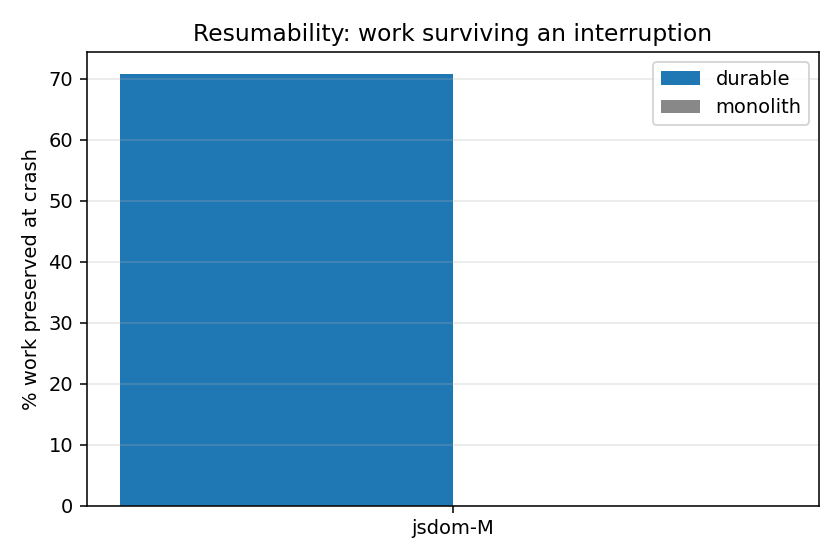
\includegraphics[width=0.62\linewidth,height=\textheight,keepaspectratio,alt={Work surviving a hard interruption at an equal wall budget (jsdom-M, 24 modules). Durable's per-layer commits preserve 70.8\% of the work as a consistent, oracle-passing partial tree it can resume from; the monolith persists nothing until one terminal write, so the interrupt loses the entire shot.}]{../figures/resumability.png}
\caption{Work surviving a hard interruption at an equal wall budget
(jsdom-M, 24 modules). Durable's per-layer commits preserve 70.8\% of
the work as a consistent, oracle-passing partial tree it can resume
from; the monolith persists nothing until one terminal write, so the
interrupt loses the entire shot.}
\end{figure}

Durable committed 17 modules across 6 dependency layers before the
interrupt (Fig. 2); resuming from that on-disk committed state completed
the remaining 7 and the tree passed the full oracle. The monolith
persists nothing until one terminal write, so its interrupted 24-file
partial tree is inconsistent, fails the oracle, and yields zero
known-good modules: the entire single shot is lost. This is a
\emph{structural} property of single-transcript execution, not a tuning
artifact: there is no mechanism by which a monolith can expose a
consistent intermediate checkpoint.

\subsubsection{4.6 Hypothesis scorecard (calibrated, including
refutations)}\label{hypothesis-scorecard-calibrated-including-refutations}

We pre-registered five hypotheses and report verdicts honestly,
including where our own headline hypothesis was \emph{refuted}, which
sharpened the contribution.

{\def\LTcaptype{none} % do not increment counter
\begin{longtable}[]{@{}
  >{\raggedright\arraybackslash}p{(\linewidth - 6\tabcolsep) * \real{0.2500}}
  >{\raggedright\arraybackslash}p{(\linewidth - 6\tabcolsep) * \real{0.2500}}
  >{\raggedright\arraybackslash}p{(\linewidth - 6\tabcolsep) * \real{0.2500}}
  >{\raggedright\arraybackslash}p{(\linewidth - 6\tabcolsep) * \real{0.2500}}@{}}
\toprule\noalign{}
\begin{minipage}[b]{\linewidth}\raggedright
H
\end{minipage} & \begin{minipage}[b]{\linewidth}\raggedright
claim (pre-registered)
\end{minipage} & \begin{minipage}[b]{\linewidth}\raggedright
verdict
\end{minipage} & \begin{minipage}[b]{\linewidth}\raggedright
evidence
\end{minipage} \\
\midrule\noalign{}
\endhead
\bottomrule\noalign{}
\endlastfoot
\textbf{H1} & a single transcript's pass-rate \emph{collapses} once
scope exceeds the window & \textbf{REFUTED (naive form) → REFRAMED} &
monolith clean to \textbf{240} modules by navigating the filesystem; it
does crack at \textbf{364}, but by \emph{capacity} (un-narrowed types),
not window-overflow. The binding constraint is \textbf{state
architecture, not nominal context length}: the paper's actual thesis. \\
\textbf{H2} & durable accumulation \textgreater{} stateless retrieval,
same decomposition+retrieval & \textbf{SUPPORTED} & durable PASS vs RAG
FAIL at S (0/3 seeds), M, L. Only accumulation differs. \\
\textbf{H3} & failure mechanism differs by architecture &
\textbf{SUPPORTED (revised)} & not generic ``context overflow'': RAG
fails by \emph{conflict} (\texttt{TS2451} only in RAG), monolith by
\emph{capacity} (\texttt{TS2571} only in monolith), durable by
neither. \\
\textbf{H4} & durable resumes near-free under interruption; transcript
must restart & \textbf{SUPPORTED} & durable 70.8\% preserved +
resume→oracle PASS; monolith 0\% preserved, full redo. \\
\textbf{H5} & a larger-window model only postpones transcript collapse &
\textbf{NOT TESTED / MOOT} & model held constant by design; the
breaking-point analysis shows window was not the binding constraint, so
the larger-window framing is superseded by H1's reframing. \\
\end{longtable}
}

That H1's naive form failed is the most important honesty in this paper:
it is \emph{why} the contribution is ``state architecture, not context
length,'' not ``we beat the context window.'' The win is concentrated
exactly where a single context is structurally insufficient (parallel
decomposition without conflicts, and resumable consistent checkpoints),
not in out-muscling a navigating agent at moderate scale.

\subsubsection{4.7 Re-query cost: zero LLM calls (the asset property,
made
literal)}\label{re-query-cost-zero-llm-calls-the-asset-property-made-literal}

The defining property of an \emph{asset} versus a \emph{prompt} is that
reuse cost → 0. Durable state has it exactly: once a discovery is
\textbf{materialized as an artifact}, recalling it is a database read:
\textbf{zero LLM invocations}. On a completed conversion job, the full
structured result (gate verdict, changed files, strict-typecheck
outcome, and the provenance that it reused a sibling's exported types)
recalls in \textbf{\textless0.5 s with no model call}. We report the
cross-arm re-query cost in \textbf{invocations}, not tokens,
sidestepping the unreliable Cursor-SDK token counts with a categorical
metric:

{\def\LTcaptype{none} % do not increment counter
\begin{longtable}[]{@{}
  >{\raggedright\arraybackslash}p{(\linewidth - 4\tabcolsep) * \real{0.3333}}
  >{\raggedright\arraybackslash}p{(\linewidth - 4\tabcolsep) * \real{0.3333}}
  >{\raggedright\arraybackslash}p{(\linewidth - 4\tabcolsep) * \real{0.3333}}@{}}
\toprule\noalign{}
\begin{minipage}[b]{\linewidth}\raggedright
arm
\end{minipage} & \begin{minipage}[b]{\linewidth}\raggedright
cost to re-query a prior discovery
\end{minipage} & \begin{minipage}[b]{\linewidth}\raggedright
why
\end{minipage} \\
\midrule\noalign{}
\endhead
\bottomrule\noalign{}
\endlastfoot
\textbf{durable} & \textbf{0 invocations} (artifact read) & discoveries
are durable system objects \\
transcript & retain in-context (window-capped → fails at scale)
\textbf{or} ≥1 (re-derive) & discoveries are transient text \\
stateless-RAG & ≥1 invocation every time & re-retrieve + re-reason;
nothing accumulates \\
\end{longtable}
}

DRR (§4.4) is the \emph{empirical rate} of these zero-cost reuses: at
the 364-module capstone, \textbf{86/293 dependency-bearing modules
(29\%)} consumed a prior worker's materialized artifact. \textbf{Honest
boundary:} ``zero'' is for \emph{recall} of an already-materialized
result; a re-query needing genuinely new synthesis still pays the
synthesis, but it starts from the artifact (no re-derivation of the
base), strictly cheaper than transcript or RAG. For \emph{this} task the
materialized discovery is a \texttt{.ts} file on disk, so a navigating
agent can also re-read it cheaply (§5); the property is most decisive
for \textbf{non-code reasoning artifacts} (analyses, decisions, traces)
that do not live in the tree, flagged as the highest-value
generalization.

\subsubsection{4.8 Parallel headroom grows with scale, but usable
concurrency is
platform-capped}\label{parallel-headroom-grows-with-scale-but-usable-concurrency-is-platform-capped}

Decomposition exposes parallelism, and the \emph{available} parallelism
\textbf{grows with repo size}: the dependency critical path (longest
chain that must run serially) shrinks as a fraction of total work as the
DAG broadens (max layer width 5 → 78 across the sweep):

{\def\LTcaptype{none} % do not increment counter
\begin{longtable}[]{@{}lll@{}}
\toprule\noalign{}
scope & critical path / total work & dataflow speedup headroom \\
\midrule\noalign{}
\endhead
\bottomrule\noalign{}
\endlastfoot
8 & 45\% & 2.2× \\
24 & 21\% & 4.8× \\
60 & 20\% & 4.9× \\
\textbf{364} & \textbf{4.6\%} & \textbf{21.6×} \\
\end{longtable}
}

\begin{figure}
\centering
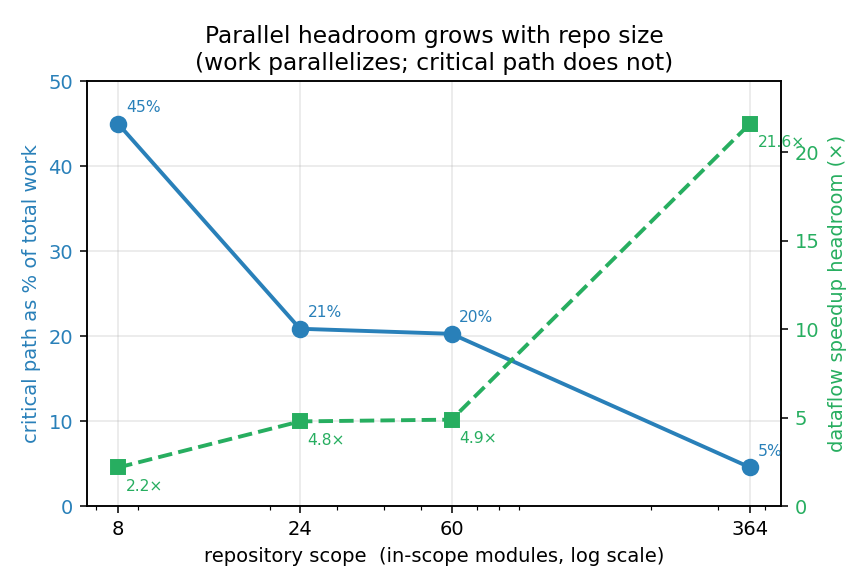
\includegraphics[width=0.72\linewidth,height=\textheight,keepaspectratio,alt={Parallel headroom grows with repository size: as the dependency DAG broadens, the serial critical path falls from 45\% of total work at 8 modules to 4.6\% at the full 364-module tree, so the theoretical dataflow speedup rises to 21.6×. Work parallelizes; the critical path does not.}]{../figures/headroom_vs_scale.png}
\caption{Parallel headroom \emph{grows} with repository size: as the
dependency DAG broadens, the serial critical path falls from 45\% of
total work at 8 modules to 4.6\% at the full 364-module tree, so the
theoretical dataflow speedup rises to 21.6×. Work parallelizes; the
critical path does not.}
\end{figure}

So \textasciitilde95\% of full-scale work is parallelizable (Fig. 3).
But a \textbf{replicated concurrency sweep} on the \emph{same}
full-scale (364-module) durable run found a hard limit that is
\textbf{not} durable state's. Each point is the mean ± 95\% CI over
n=5--10 quality-gated replicates, all measured with an \emph{identical}
protocol: a fixed 240 s steady-state window per run, every run
contamination-checked (\texttt{base\_build\_start==1}) and required to
complete the full window (Fig. 4). Worker success is high below the cap
(C=8 → 97\% ±5.7, C=12 → 99\% ±2.0) and \textbf{collapses monotonically}
through a sharp knee (C=16 → 66\% ±2.7, C=24 → 28\% ±4.3, C=32 → 19\%
±8.1); the excess sessions are throttled into fast (\textless20 s vs
\textasciitilde90--170 s) no-edit returns. Reading the \textbf{effective
admission cap} off the knee gives \textbf{K≈10--12} (C=12 K\_eff=11.9,
C=16 K\_eff=10.5). Above the cap the rate falls \emph{below} a
\texttt{min(1,\ K/C)} reference: retry churn on throttled sessions
inflates the denominator, so the collapsed regime is \emph{steeper} than
1/C.

\begin{figure}
\centering
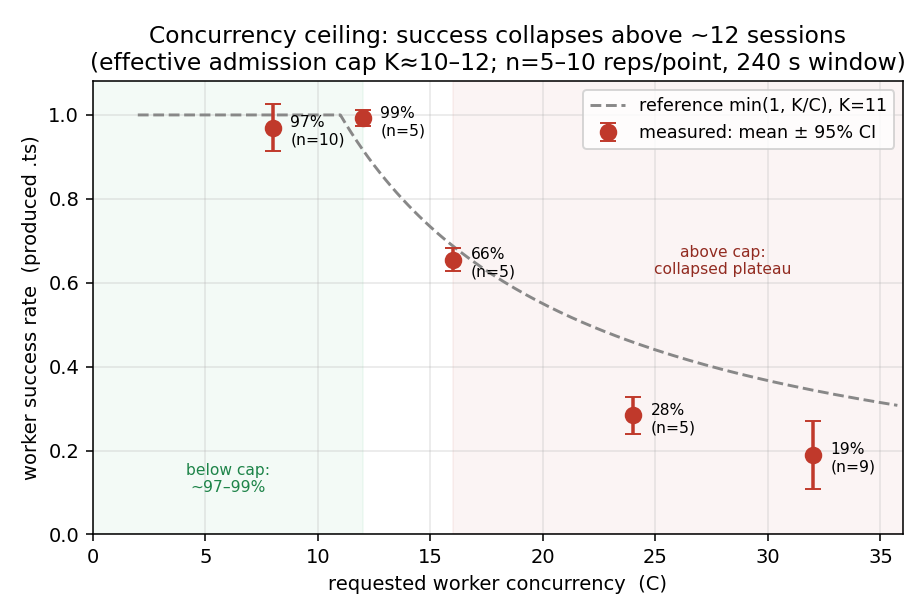
\includegraphics[width=0.78\linewidth,height=\textheight,keepaspectratio,alt={Replicated concurrency sweep on the full-scale (364-module) durable run, Cursor backend (n=5--10 per point, uniform 240 s window, mean ± 95\% CI). Worker success holds at \textasciitilde97--99\% below \textasciitilde12 simultaneous sessions and collapses monotonically above it: an effective admission cap of K≈10--12 imposed by the serving API, which durable state + retry then absorbs.}]{../figures/concurrency_ceiling.png}
\caption{Replicated concurrency sweep on the full-scale (364-module)
durable run, Cursor backend (n=5--10 per point, uniform 240 s window,
mean ± 95\% CI). Worker success holds at \textasciitilde97--99\% below
\textasciitilde12 simultaneous sessions and collapses monotonically
above it: an effective admission cap of K≈10--12 imposed by the serving
API, which durable state + retry then absorbs.}
\end{figure}

(An earlier single-run probe showed a spurious non-monotonicity at C=24;
replication with the uniform-window protocol showed it was a measurement
artifact of mixed stop-rules, not a property of the system.) We
attribute the cap to the \textbf{Cursor API/SDK, not the orchestrator}:
Puppetmaster spawned, leased, and retried every worker correctly, and
durable state + retry \emph{absorbed} the throttle (the run still
converges). \textbf{We confirm this with a second-backend control} (Fig.
5): holding the orchestrator and durable state fixed and swapping only
the worker backend from Cursor agents to \textbf{Claude Code} (Anthropic
API), a concurrency probe that launches exactly C workers simultaneously
sustains \textbf{100\% success at every C ∈ \{4,8,16,24,32\}} (n=3 each;
252 workers; 0 fast-fails), including at C=16/24/32, where the Cursor
backend collapses to 66\%/28\%/19\%. The contrast is the result:
identical orchestration + durable state, one backend caps and the other
does not, so the cap is a property of the \textbf{serving platform}, not
of durable state or the orchestrator. (We keep both arms precisely
because the platform-specificity claim \emph{is} this contrast; a
single-backend curve could not establish it.)

\begin{figure}
\centering
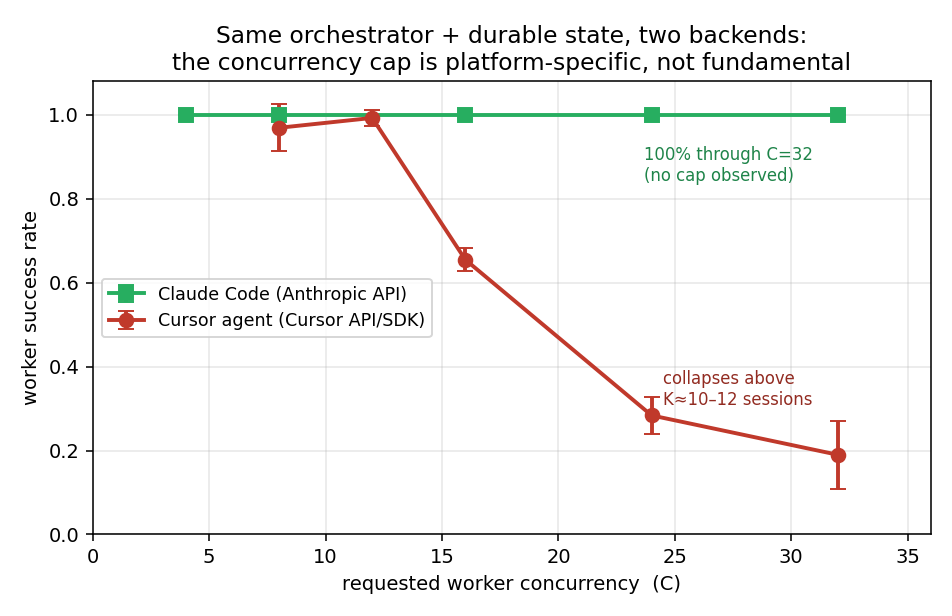
\includegraphics[width=0.8\linewidth,height=\textheight,keepaspectratio,alt={The same orchestrator and durable state on two serving backends. The Cursor backend (red) collapses above its K≈10--12 session cap; the Claude Code backend (green) sustains 100\% worker success through C=32 (n=3 per point, 252 workers, 0 fast-fails). The concurrency cap is therefore platform-specific, not a property of durable state.}]{../figures/concurrency_backends.png}
\caption{The same orchestrator and durable state on two serving
backends. The Cursor backend (red) collapses above its K≈10--12 session
cap; the Claude Code backend (green) sustains 100\% worker success
through C=32 (n=3 per point, 252 workers, 0 fast-fails). The concurrency
cap is therefore platform-specific, not a property of durable state.}
\end{figure}

The consequence: at the practical ceiling, durable wall ≈
work/\textasciitilde11 ≈ 1.1 h vs the monolith's 0.83 h, so durable is
\textasciitilde1.3× \emph{slower} on wall-clock while being the only arm
that reaches a clean strict typecheck at full scale. The 21.6×
theoretical headroom is real but only \textasciitilde K of it is
spendable at once today; closing that gap is an \emph{orchestration}
problem (§6 future work), not a property of durable state.

\subsection{5. Discussion}\label{discussion}

\begin{itemize}
\tightlist
\item
  \textbf{Three advantages, one root.} Everything durable wins flows
  from a single property, \emph{discoveries are durable system objects,
  not disposable prompt text}: (1) conflict-free parallel decomposition
  (§4.2--4.3); (2) interruption-resumable consistent checkpoints (§4.5);
  (3) zero-marginal-cost re-query of materialized discoveries (§4.7).
\item
  What durable state does \textbf{not} buy for \emph{this} task: raw
  single-agent navigation is already strong at moderate scale, and
  because the migration artifact is code on disk, re-reading a prior
  discovery is filesystem-cheap for any navigating agent too, so the
  zero-cost-re-query advantage is \emph{under-tested} here and is most
  decisive for non-code reasoning artifacts. We do not claim otherwise.
\item
  Implication: the durable advantage is an
  \emph{orchestration/coordination} property, realized when one context
  is insufficient, or work must survive interruption, parallelize, or be
  revisited cheaply, not a universal ``context is solved'' claim.
\item
  \textbf{The speed gap is an orchestration ceiling, not a
  state-architecture one.} Durable's \textasciitilde1.3× wall-clock
  penalty at full scale (§4.8) is set by a \emph{platform} session cap
  (K≈10--12 on Cursor), not by accumulation. We demonstrate this
  directly: the same orchestrator and durable state on a \textbf{second
  backend (Claude Code) sustains 100\% to C=32} where Cursor collapses
  (Fig. 5). The theoretical 21.6× headroom says the \emph{architecture}
  scales; realizing it is an engineering problem on the
  serving/scheduling side (§6), and the backend choice alone moves the
  ceiling.
\end{itemize}

\subsection{6. Threats to validity}\label{threats-to-validity}

\begin{itemize}
\tightlist
\item
  \textbf{jsdom build-system coupling (scope-correlated).} jsdom's
  \texttt{npm\ run\ prepare} runs \texttt{scripts/webidl/convert.js},
  which \texttt{require()}s
  \texttt{lib/jsdom/living/helpers/namespaces.js} by \emph{literal
  \texttt{.js} path}. On any trial whose scope includes that one helper,
  converting it to \texttt{.ts} makes jsdom's own IDL codegen fail,
  which fails the \emph{runtime} gate (\texttt{tests\_api}). We verified
  this is \emph{exactly} scope-membership-correlated (L-durable-s2 with
  namespaces.js ∈ scope hit it; L-durable-s1 without it did not, same
  L(60) scale): a target build artifact, arm-independent, not a
  durable-arm defect and not a scale effect. We therefore make affected
  comparisons on the \textbf{static} axis (\texttt{typecheck\_strict} +
  \texttt{escape\_hatches}), which jsdom's build cannot perturb, and
  flag \texttt{tests\_api} as confounded on those trials. A
  codegen-baked harness (run \texttt{prepare} on the pristine tree
  pre-conversion, exclude \texttt{scripts/} from scope) removes the
  confound; logged as future work rather than silently dropped.
\item
  One task family (migration); artifact == code. Generalization to
  reasoning-artifact tasks is future work.
\item
  Oracle hardening history (hollow passes, subprocess \texttt{.ts}
  loading, over-broad hatch counting): all trees re-scored by the final
  oracle for internal consistency; the hatch fix flipped mono-240 from a
  false FAIL to its true PASS.
\item
  Cursor-SDK token counts are unreliable (implausibly low); we report
  wall-clock, worker count, and DRR as the cost axes instead of token
  deltas.
\item
  Main results run on a single platform (Puppetmaster Cursor workers)
  with model routing held constant; §4.8 adds a Claude Code backend as a
  control for the concurrency claim only.
\item
  \textbf{Platform concurrency ceiling (§4.8).} On the Cursor backend,
  usable parallelism is capped at an effective K≈10--12 concurrent agent
  sessions by the serving API, so the measured Cursor wall-clock does
  not yet realize the 21.6× dataflow headroom. This bounds the
  \emph{speed} comparison (Cursor durable \textasciitilde1.3× the
  monolith at full scale) but not the \emph{correctness},
  \emph{resumability}, or \emph{re-query} results, none of which depend
  on concurrency. We ran a \textbf{replicated} sweep at
  C∈\{8,12,16,24,32\} (n=5--10 per point, uniform 240 s window, every
  run contamination-checked and quality-gated for a complete window),
  mean ± 95\% CI; the collapse is monotone and tightly resolved.
  Crucially, a \textbf{second backend (Claude Code / Anthropic) under
  the same orchestrator sustains 100\% to C=32} (Fig. 5), so the cap is
  platform-specific, not fundamental: it is an orchestration/serving
  constraint, not a property of durable state.
\end{itemize}

\subsection{6.1 Future work (orchestration track, distinct from the
state-architecture
claim)}\label{future-work-orchestration-track-distinct-from-the-state-architecture-claim}

These close the §4.8 speed gap and are properties of the
\emph{scheduler/serving layer}, not of durable state; we list them so
the speed result is not mistaken for a ceiling on the architecture:

\begin{itemize}
\tightlist
\item
  \textbf{Adaptive admission control.} Cap dispatch near the observed
  session ceiling instead of launching \texttt{max\_workers} that mostly
  fast-fail; treat a burst of sub-N-second no-edit returns as
  backpressure and throttle, eliminating wasted API calls beyond K.
\item
  \textbf{Throttle-vs-failure classification.} A sub-N-second
  \texttt{require\_diff} failure should re-queue as backpressure, not
  count against a task's quality budget (no retry storms).
\item
  \textbf{Dataflow scheduling.} Release a module the instant its
  dependencies commit, rather than at full-layer barriers; the
  theoretical critical-path floor is 0.55 h \textless{} the monolith's
  0.83 h, so dataflow + a higher session allowance is the path to a
  \emph{speed} win, not just parity.
\item
  \textbf{Non-code reasoning-artifact tasks} to test the zero-cost
  re-query advantage (§4.7) where the discovery does not live on the
  filesystem.
\end{itemize}

\subsection{7. Conclusion}\label{conclusion}

Repository-scale agent performance is primarily constrained by
\textbf{state architecture}, not nominal context length. A single modern
agentic context scales much further than the context-length arms race
assumes (clean to 240 modules by navigating the filesystem), but it does
eventually crack at full-repo scale, and it cracks by \emph{capacity}
(un-narrowed types under one global view), not by running out of window.
When work is decomposed for parallelism or resilience, \emph{how state
flows between workers} becomes decisive: stateless retrieval fails by
\emph{conflict} (colliding declarations its blind workers cannot
reconcile), while durable accumulation fails by neither, additionally
buying interruption-resumable consistent checkpoints. The win comes from
treating discoveries as durable, consistent, reusable system objects ---
\emph{state is an asset, not a prompt}.

\subsection{References}\label{references}

\begin{itemize}
\tightlist
\item
  Lewis, P., Perez, E., Piktus, A., Petroni, F., Karpukhin, V., Goyal,
  N., Küttler, H., Lewis, M., Yih, W., Rocktäschel, T., Riedel, S., \&
  Kiela, D. (2020). \emph{Retrieval-Augmented Generation for
  Knowledge-Intensive NLP Tasks.} NeurIPS 2020. arXiv:2005.11401.
\item
  Liu, N. F., Lin, K., Hewitt, J., Paranjape, A., Bevilacqua, M.,
  Petroni, F., \& Liang, P. (2023). \emph{Lost in the Middle: How
  Language Models Use Long Contexts.} TACL 2024. arXiv:2307.03172.
\item
  Zhang, F., Chen, B., Zhang, Y., Keung, J., Liu, J., Zan, D., Mao, Y.,
  Lou, J.-G., \& Chen, W. (2023). \emph{RepoCoder: Repository-Level Code
  Completion Through Iterative Retrieval and Generation.} EMNLP 2023.
  arXiv:2303.12570.
\item
  Shinn, N., Cassano, F., Berman, E., Gopinath, A., Narasimhan, K., \&
  Yao, S. (2023). \emph{Reflexion: Language Agents with Verbal
  Reinforcement Learning.} NeurIPS 2023. arXiv:2303.11366.
\item
  Packer, C., Wooders, S., Lin, K., Fang, V., Patil, S. G., Stoica, I.,
  \& Gonzalez, J. E. (2023). \emph{MemGPT: Towards LLMs as Operating
  Systems.} arXiv:2310.08560.
\item
  Jimenez, C. E., Yang, J., Wettig, A., Yao, S., Pei, K., Press, O., \&
  Narasimhan, K. (2023). \emph{SWE-bench: Can Language Models Resolve
  Real-World GitHub Issues?} ICLR 2024. arXiv:2310.06770.
\end{itemize}

\end{document}
